\chapter{Designing and testing of Helmholtz Coil}


We constructed a Helmholtz coil inorder to test the detumbling system developed for our cubesat. Using Helmholtz coil a constant and uniform magnetic field is generated. Here we produced magnetic field greater than earth magnetic field to achieve detumbling at faster rate.

\subsection{Objective}

The magnetotorquer in the actual cubesat produces the opposite torque depending on the earth's magnetic field. Since earth's magnetic field is in the range of microteslas and hence it takes hours to stabilize the cubesat. But in the prototype of the cubesat we should demonstrate the detumbling process in a much lesser time. Inorder to achieve this task we provide a bigger magnetic field value in the order of milliteslas so the detumbling process occurs at a greater speed. The optimum value of magnetic moment was fixed as 1 millitesla keeping residual angular velocity low and achieving detumbling within few minutes. This is obtained by modifying the aforementioned CubeSat simulation script. We have to design a Helmholtz coil which generates the required magnetic field.

\subsection{Theoretical Calculations}
\par The formula used to calculate the theoretical value of magnetic field at the centre of two coils is given below

$$ B= \frac{8}{5\sqrt{5}}\frac{\mu_0 NI}{R}$$\\
\hspace{100pt} (Derived equation of magnetic field at centre of Helmholtz \ref{magneticfield})\\

Where n = number of turns
            I = current(measured using multi meter)
            R = radius of the Helmholtz coil.
\vspace{10pt}  

For accomodating the CubeSat along with the airbearing inside the Helmholtz cage, we've alotted a gap of 26cm between the Coils. Therefore the radius of the Helmoltz coils should also be made to be equal to 26cm for maintaining uniform magnetic field at the midpoint of the two helmholtz cols. The cage needs to be fabricated as per the dimensions given below \ref{fig-hlmhtz-cad}.

\begin{figure}[h!]
	\centering
	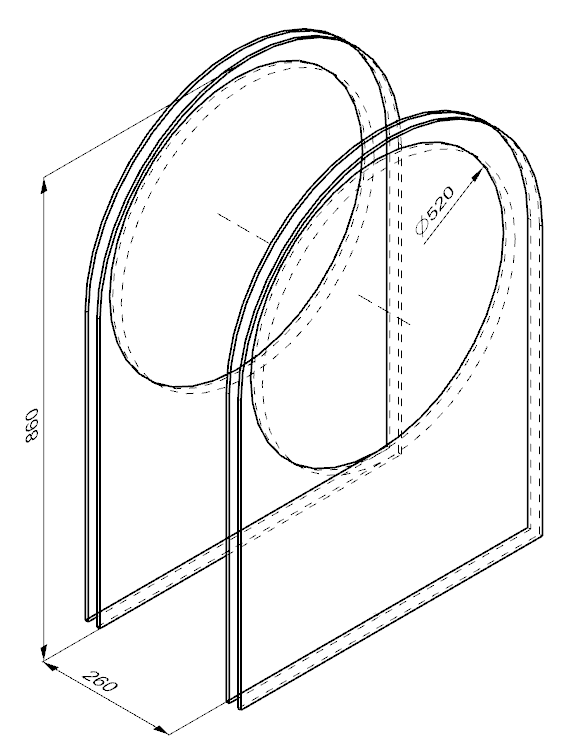
\includegraphics[width=4in,height=4in]{./images/assem.png}
	\caption{Model of the Helmholtz cage}
	\label{fig-hlmhtz-cad}
\end{figure}

The magnetic field produced by the Helmholtz coil also depends upon number of turns and the current through the coil. The resistance per unit length depends upon the gauge of the wire used. So we have to fix the gauge of wire, value of current and number of turns in a perfect combination so as to achieve desired power draw. If we decrease the gauge of wire, thickness increases and we get less power draw but when thickness increases winding coil becomes difficult.We also limited the number of turns so that we are able to hand wind the coil. 

To acheive this we wrote a script in Matlab that iterates between different guages of wire and different number of turns to find the current, power draw etc for each combination.\\

\noindent For 10SWG,

\noindent N = 50, I = 5.8A and P = 5.76W (obtained from \ref{helmeqn})

\noindent N = 51, I = 5.7A and P = 5.66W

\noindent ......

\noindent N = 200, I = 1.45A and P = 1.43W\\

\noindent For 11SWG,

\noindent N = 50, I = 5.8A and P = 7W

\noindent ......

\noindent N = 200, I = 1.45A and P = 1.75W\\

\noindent For 12SWG,

\noindent N = 50, I = 5.8A and P = 8.7W

\noindent ......

\noindent N = 200, I = 1.45A and P = 2.17W\\

\noindent and so on...\\

We found an optimum combination of 14SWG Copper wire with 150 turns and 1.966A \ref{fig-helm-vals} that produces the required magnetic field.\\

\begin{figure}[h!]
	\centering
	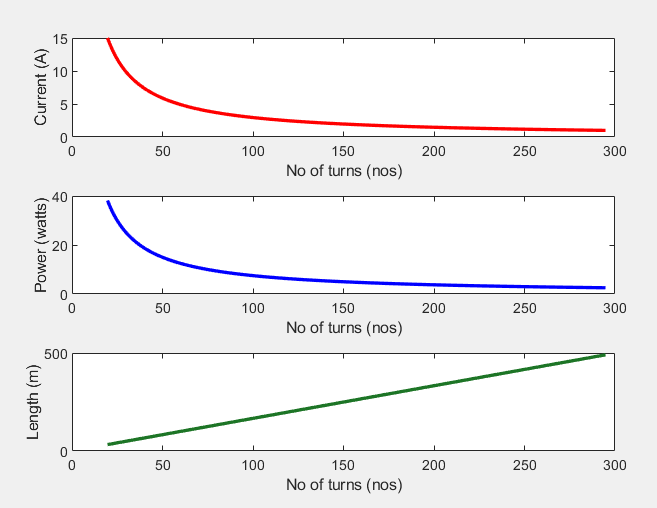
\includegraphics[width=4in,height=2.8in]{images/14swg.png}
	\caption{Current and Power draw for 14SWG wire}
	\label{fig-helm-vals}
\end{figure}

\par Matlabcode used for plots:
github link- \url{https://github.com/NEONGASHMEN/arduinodemo1U/blob/main/helmholtz/hhz_vals.m}

\subsection{Miniature model of Helmholtz coil}
To check our theoretical assumptions before the fabrication of actual helmholtz coil we made a miniature model by 3D printing it with ABS(Acrylonitrile Butadiene Styrene) with diameter 10cm and winded with 28 AWG copper wire.

\par We tested it and proved that the theoretical value of the magnetic field at the centre of the two coils is equal to the practical value of magnetic field measured using EMF detector.


\subsection{Fabrication of Helmholtz coil}

A Plywood frame of aforementioned dimensions was fabricated using a woodcutter and adhesives. Plywood was choosed because of its relative permeability, which has the value close to that of air and also because it is easily available and is cheap. We wound the wire about 150 turns per coil around the plywood frameby hand. The Helmholtz coil is designed to produce 1mT magnetic field. A SMPS was used to control the voltage applied to the coil. Here we used a 12V SMPS according to our current requirement and for safety reasons.

We used a multimeter to measure the current flowing through the coil and measured the magnetic field using a magnetometer. The current was limited to 1.96A using a variable rheostat and the magnetic field was found to be xmT. The margin of error is x. The power draw was found out to be less than xW.

\vspace{10pt}
\begin{figure}[h!]
	\centering
	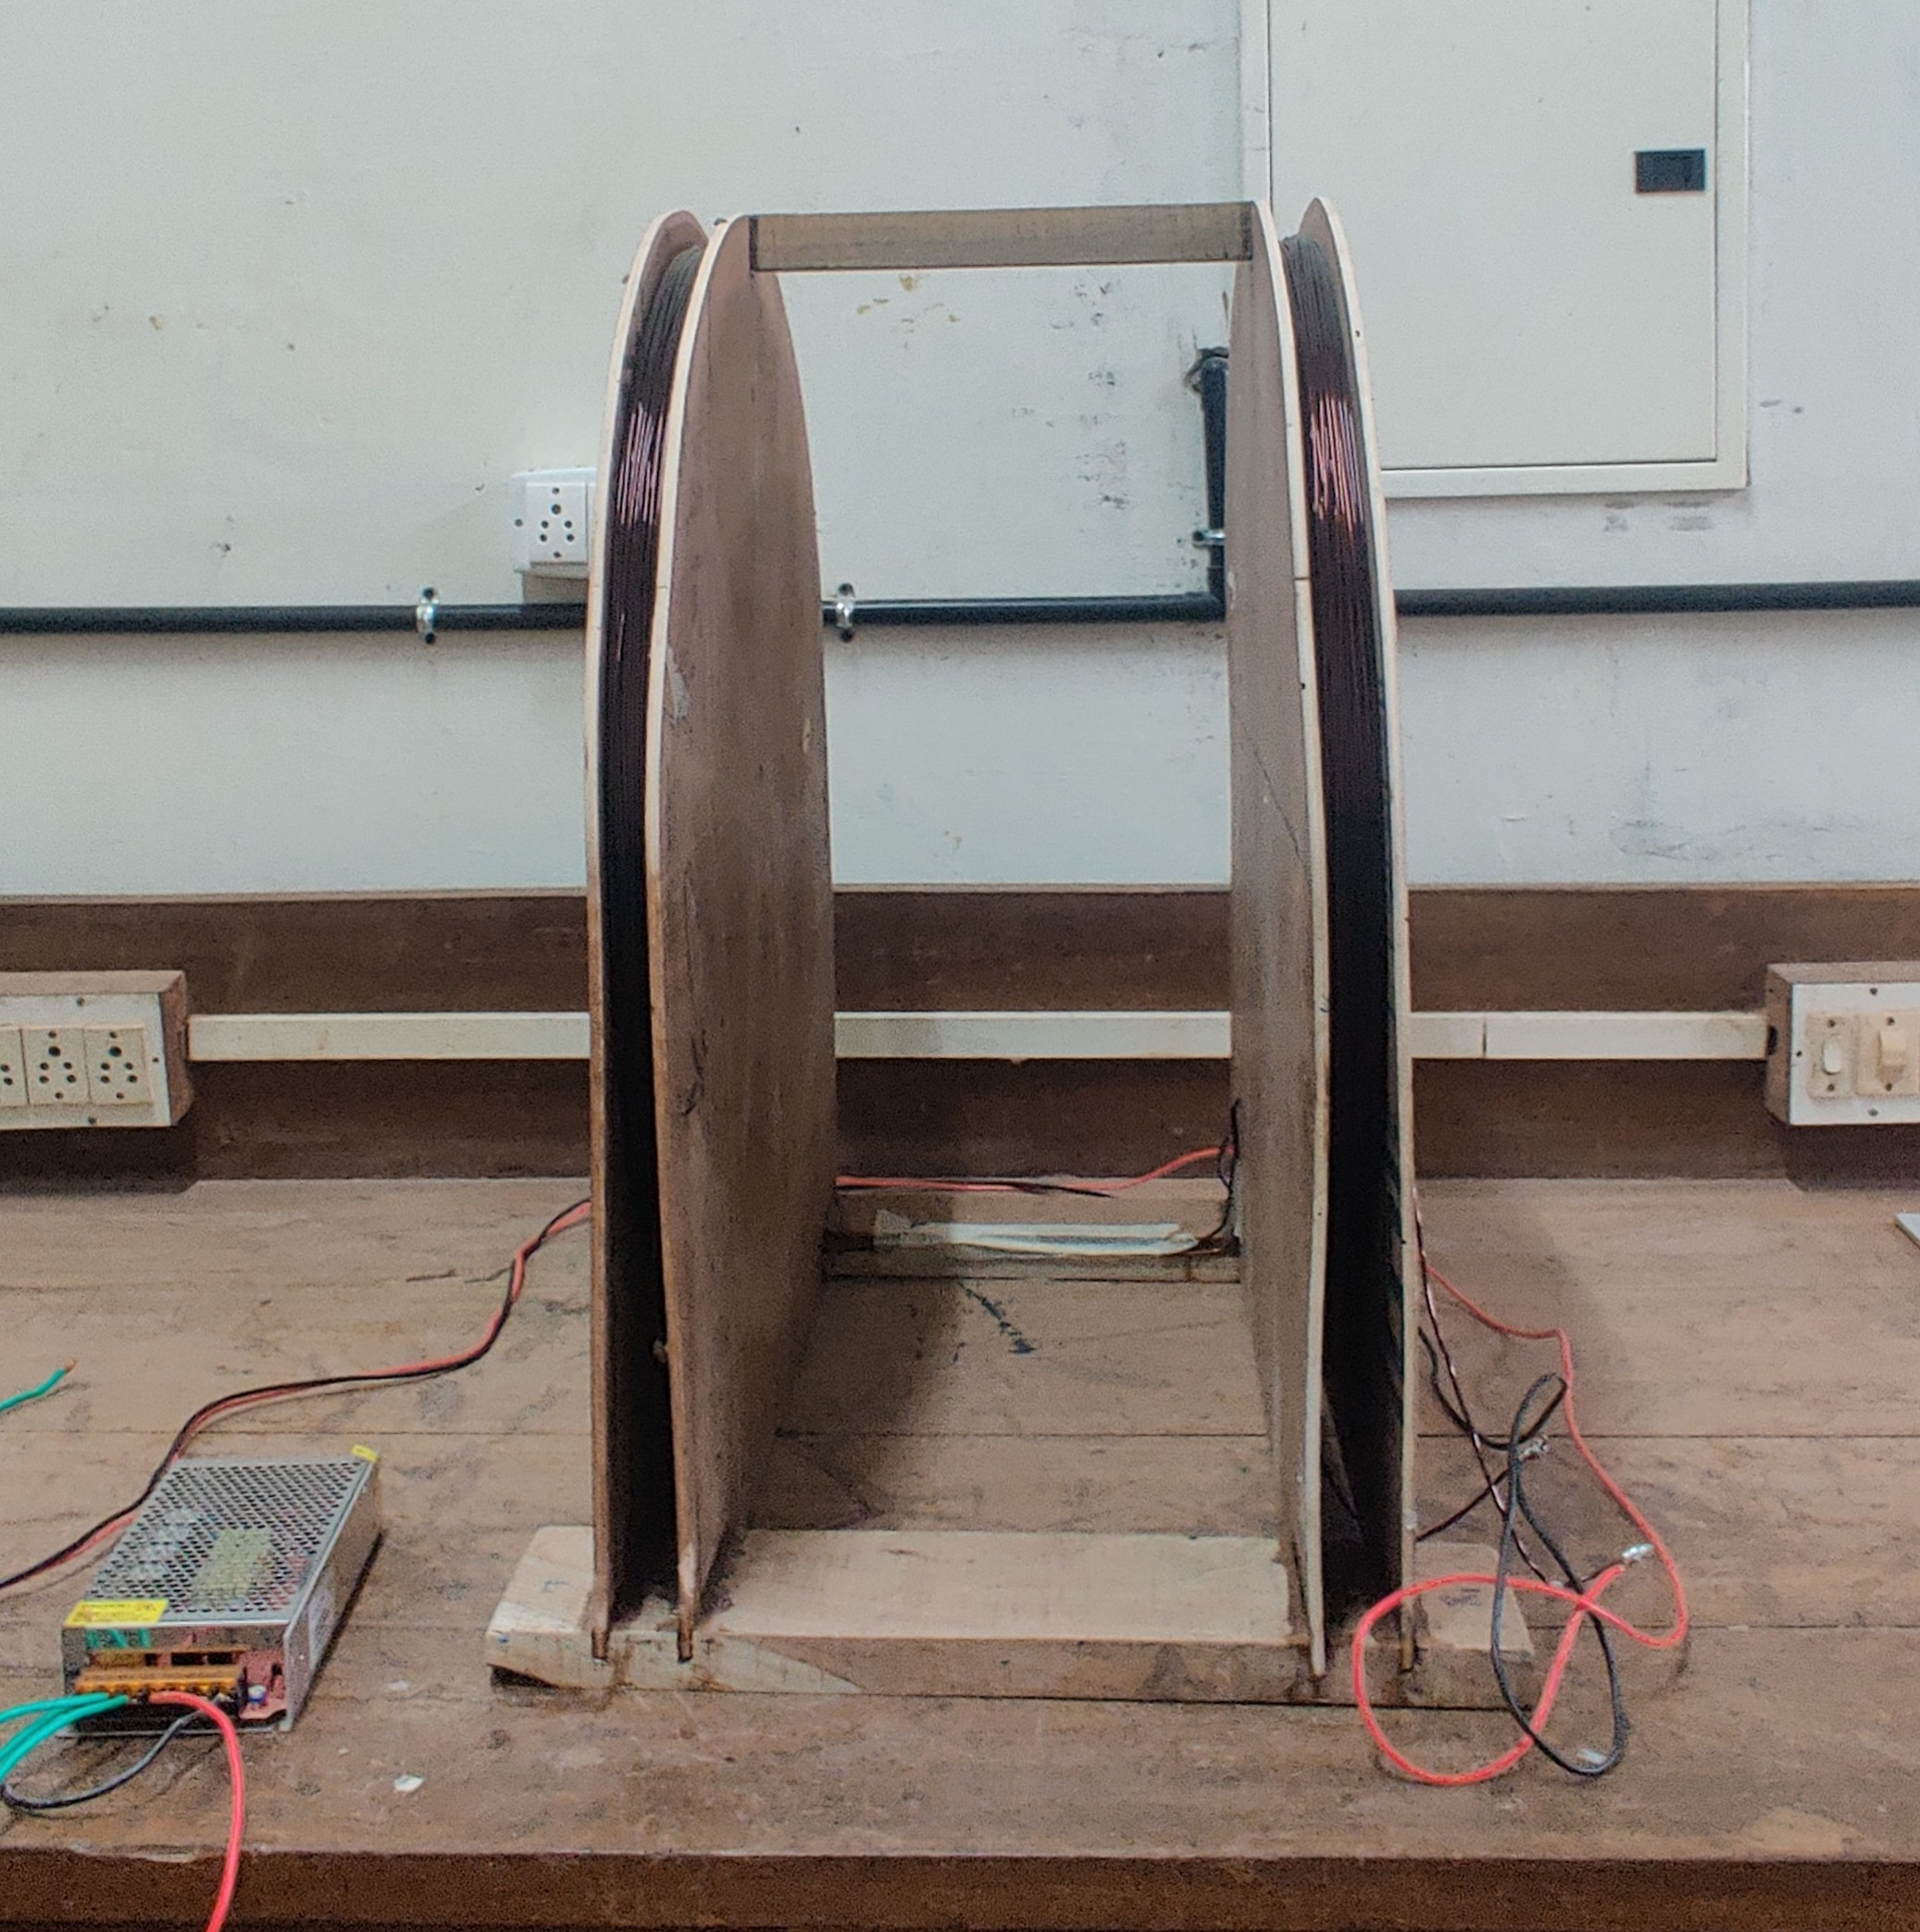
\includegraphics[width=4in,height=4in]{images/1pic.jpg}
	\caption{Helmholtz coil}
	\label{fig-wVt}
\end{figure}
